\chapter{Resultado e Discussão} \label{sec:results}

Foram identificados os 4 modelos de mundo que demonstraram maior
importância para o estudo, os mesmos estão identificados na Tabela \ref{tab:designs}.

\begin{table}[hbt]
    \centering
    \begin{tabular}{c|c|c|c}
        Modelo & Conjunto de Estados & Conjunto de Recompensas & Tamanho da Fila \\ \hline
        Modelo \customlabel{model:old}{1} & 1 & 1 & 5  \\
        Modelo \customlabel{model:2cycles}{2} & 1 & 2 & 2 \\
        Modelo \customlabel{model:1cycle}{3} & 1 & 2 & 1 \\
        Modelo \customlabel{model:simple}{4} & 2 & 2 & 5 \\ 
    \end{tabular}
    \caption{Modelos de Mundo}
    \label{tab:designs}
\end{table}

Após a execução de grande número de episódios, para treinamento dos modelos
propostos, foram separados em planilhas as quantidades de gols resultantes para
cada bloco de 3000 ciclos para cada um. A partir da execução de 500 blocos
(1.500.000 ciclos) foi feita uma
média geral, uma média dos primeiros 100 registros e uma média de apenas os
últimos 100 registros, levando em conta que se
espera que tenha havido uma melhora na defesa de cada um.

Na Tabela \ref{tab:results} estão listados os modelos de mundo e as médias calculadas e
por fim o valor para comparação do time original. Uma comparação visual é
ilustrada pela Figura \ref{img:averages}.

\definecolor{LightBlue}{rgb}{0.79,0.93,1}

\begin{table}[hbt]
    \centering
    \begin{tabular}{c|c|c|c}
        Modelo & Média Geral & Média dos primeiros 100 blocos & Média dos últimos 100 blocos \\ \hline
        Modelo \ref{model:old} & 44,08 & 44,09 & 44,11  \\
        \rowcolor{LightBlue}
        Modelo \ref{model:2cycles} & 41,48 & 40,21 & 37,82 \\
        \rowcolor{LightBlue}
        Modelo \ref{model:1cycle} & 41,75 & 44,1 & 39,03 \\
        Modelo \ref{model:simple} & 44,69 & 44,4 & 44,77 \\ \hline
        Original &  26,45\\
    \end{tabular}
    \caption{Resultados - Médias de Gols por bloco de 3000 mil ciclos.}
    \label{tab:results}
\end{table}

\imagem{.4}{averages}{Médias finais em comparação ao original}{O Autor}

A observação da Tabela \ref{tab:results} faz com que seja possível perceber que
os modelos de mundo com melhor evolução, ou alguma evolução, são os Modelos
\ref{model:2cycles} e \ref{model:1cycle}. Por conta desta observação foram
realizados um número maior de execuções nos mesmos para que fossem 
traçados gráficos (Figura \ref{img:graph}) cruzando o número de blocos executados no teste e o número de
gols sofridos no último bloco juntamente com a curva de tendência linear formada
por este cruzamento de ambos modelos para que se possa ser feito a visualização
do melhoramento dos mesmos.

\begin{figure}[!htb]
\centering
    \caption{\label{img:graph} Gráficos de Modelos \ref{model:2cycles} e \ref{model:1cycle}}
    \subcaptionbox{\label{img:2cycles} Modelo \ref{model:2cycles}}{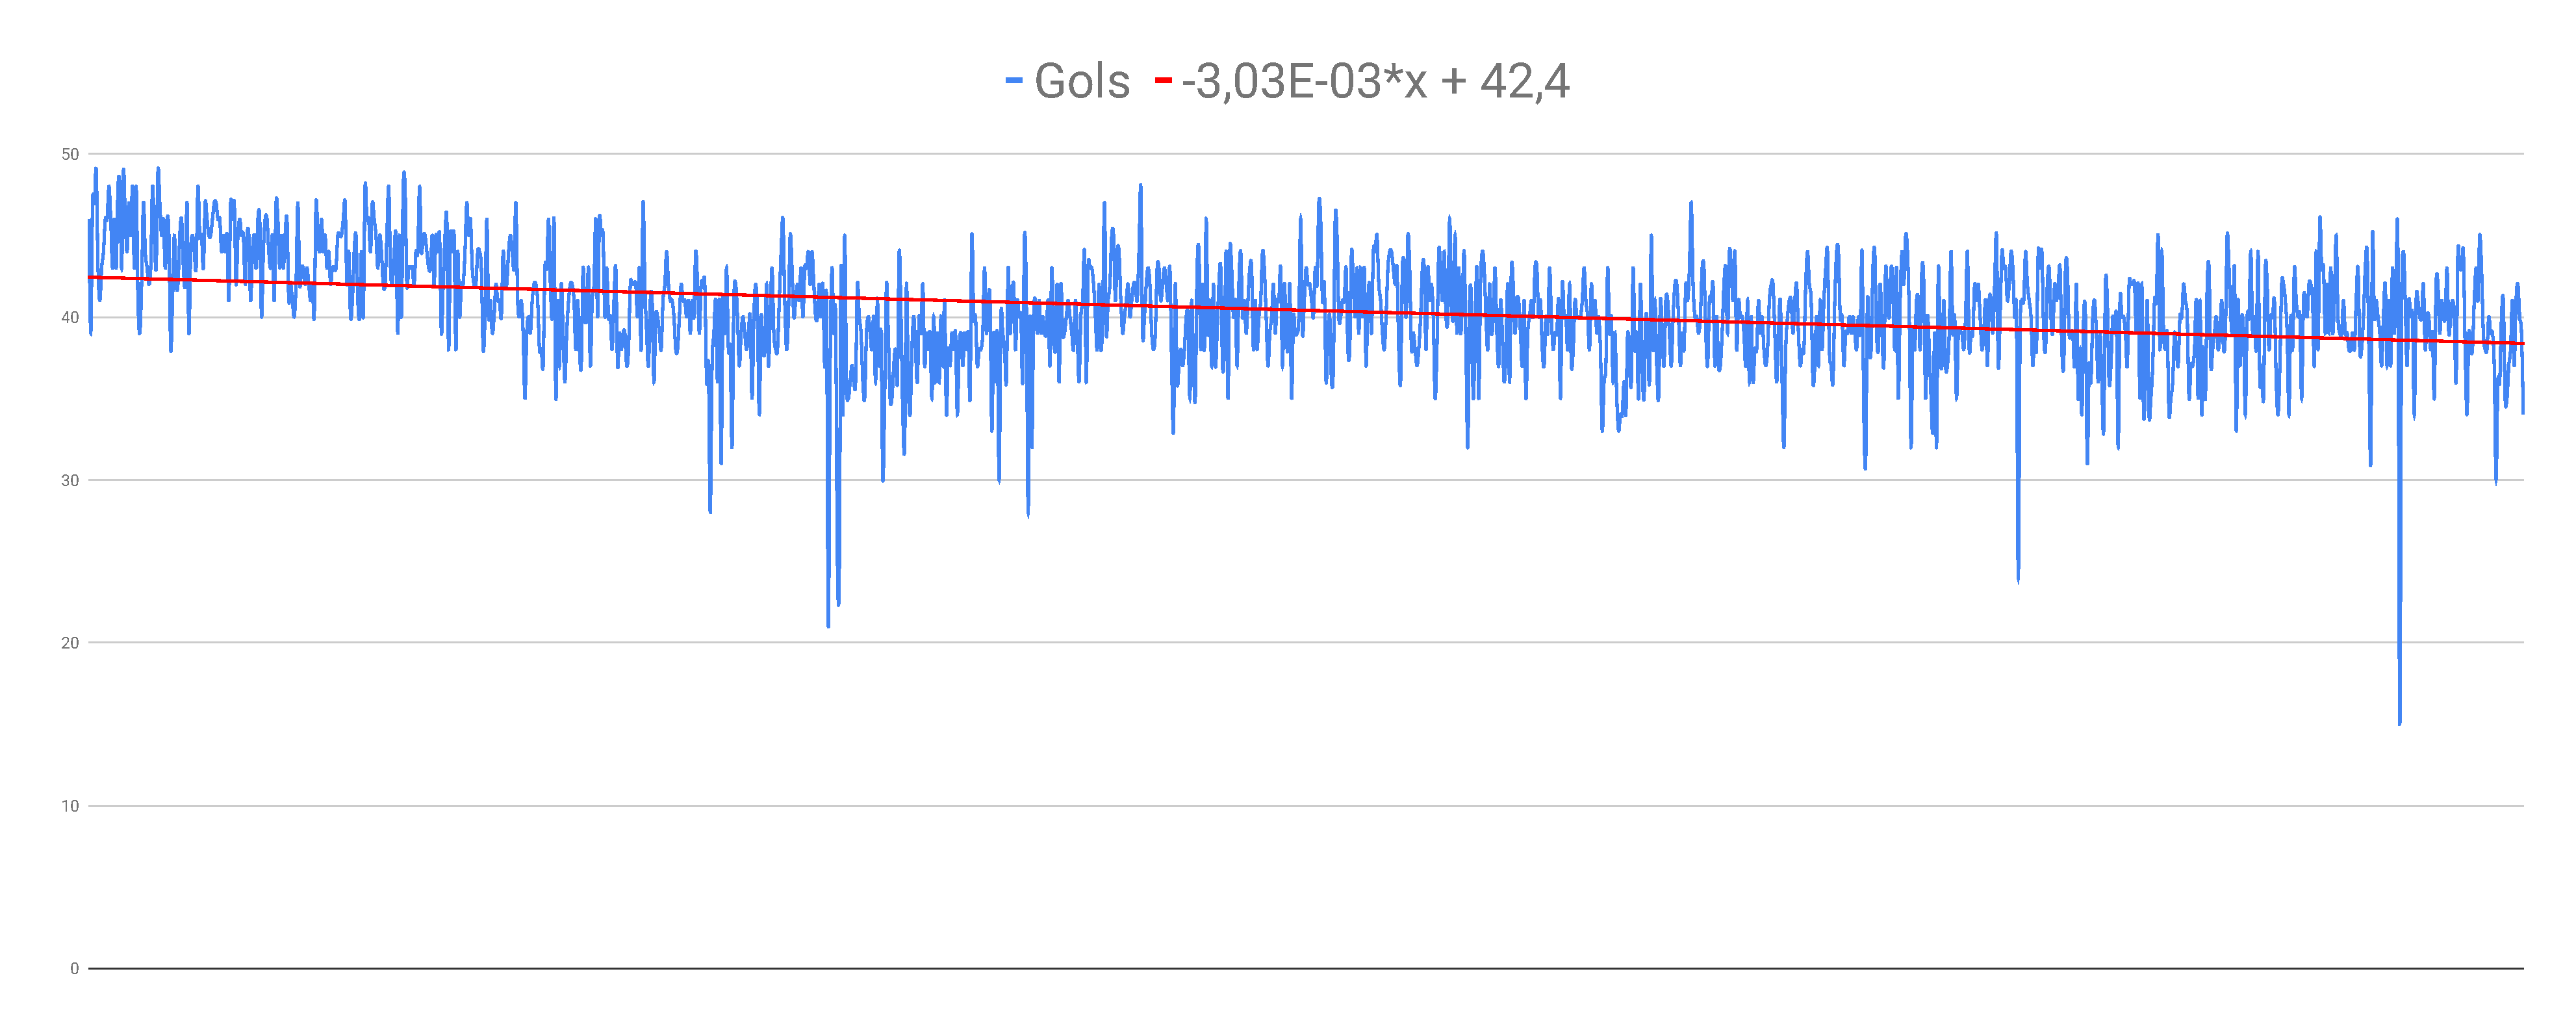
\includegraphics[scale=.235]{img/2cycles}}\qquad
    \subcaptionbox{\label{img:1cycle} Model \ref{model:1cycle}}{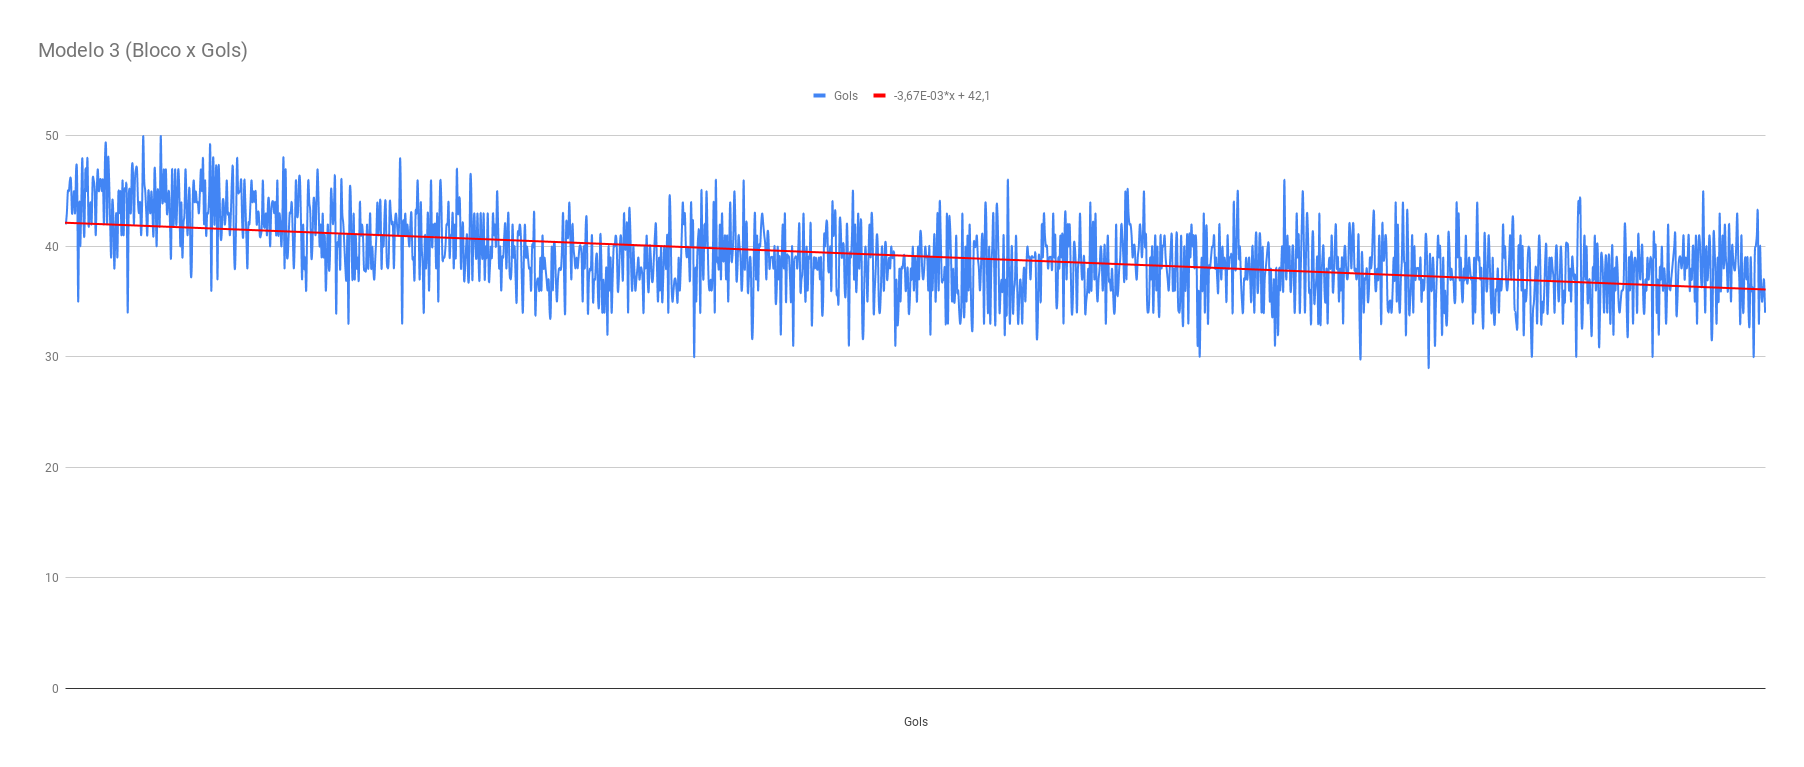
\includegraphics[scale=.25]{img/1cycle}}
    \vspace{1.5em}
    \legend{\textbf{Fonte:} O Autor}
\end{figure}

Os gráficos foram traçados com auxílio da ferramenta de planilhas Google Sheets\footnote{https://docs.google.com/spreadsheets} que
permitiu a captura da equação da curva de tendência traçada. O Modelo
\ref{model:2cycles} é representado pela equação \ref{eq:2cycles} e o Modelo
\ref{model:1cycle} é representado pela Equação \ref{eq:1cycle}, onde $G$
representa a média de gols sofridos por bloco e $b$ o número de blocos executados.

\begin{equation}
    \label{eq:2cycles}
    G=-3,03\times 10^{-3}\times b+42,4
\end{equation}

\begin{equation}
    \label{eq:1cycle}
    G=-3,67\times 10^{-3} \times b+42,1
\end{equation}

É possível observar que os gráficos dos resultados dos Modelos
\ref{model:2cycles} e \ref{model:1cycle} apresentam sinais de evolução na
inteligência dos agentes quanto a tentativa de evitar gols. A análise destes
gráficos, apresentados na Figura \ref{img:graph}, mostra um comportamento
semelhante a ruídos, o que é espererado devido , primeiro, a
característica da simulação que cria ruídos nos sensores dos agentes para que os
mesmos se assemelhem aos sensores falhos dos seres humanos e a característica
aleatória da criação de situações do sistema de treinamento.

Apesar desta observação, como demonstrado na mesma figura e nas Equações
\ref{eq:1cycle} e \ref{eq:2cycles}, que se tratam de regressões lineares dos
resultados encontrados, é possível encontrar um comportamento de melhoria nos
modelos de mundo em questão. Baseando-se em tais equações, é possível extrapolar
um possível valor para o número de blocos a ser executados para que possa ser
superado a média geral do time original, para o Modelo \ref{model:2cycles}, este
número seria de 5265 blocos (mais de 15.000.000 ciclos), já para o Modelo
\ref{model:1cycle} este número seria de 4265 blocos (mais de 12.000.000 ciclos).

É possível, ainda, observar que a tentativa de avaliar a ação tomada após alguns ciclos
de sua execução não apresentou os frutos esperados, pelo contrário, os dois
modelos em destaque foram aqueles com menor número de ações na fila, o que
indica que o melhor momento para colher os resultados de uma ação é o seguinte à
sua execução. Também é
possível observar que a primeira abordagem de estados se mostrou mais
eficiente que a segunda.